\section{MCU}\label{sec:mcu-hw}

	The choosen MCU for the system is the \textit{ATMEGA32U4} manufactured by \textit{Microchip}. According to \cite{atmega32u4-features} and \cite{atmega32u4-datasheet} the main features of this MCU are:
		\begin{itemize}
			\item{\textit{Program Memory (Flash)}}: 32KB.\label{itm:program-memory-flash}
			\item{\textit{Communication Peripherals}}: 1-USB, 1-UART, 2-SPI, 1-I2C.\label{itm:communication-peripherals}
			\item{\textit{ADC}}: 12-channels, 10-bit ADC.\label{itm:hw-mcu-adc}
			\item{\textit{Operating Voltage Range}}: 2.7 to 5.5V.\label{itm:operating-voltage-range}
		\end{itemize}
	\par
	This microcontroller family is widely used in academic environment (specially after the Arduino project started, when microncontroller programming became much more feasible and reachable), and is famous for being easy and reliable to use. The \textit{ATmega32U4} is really versatile and more important it meets this project requirements, listed in Section \ref{sec:functionalRequirements}. A very useful feature of this MCU is that it has a USB 2.0 controller built-in, this eliminates the need for a additional transceiver circuit, moreover this MCU can be easily reprogrammable through the USB port, this being a very useful feature when the hardware is fully assembled. Figure \ref{fig:atmega32u4-pinout} shows the pinout of this device.

	\begin{figure}[htbp]
		\centering
		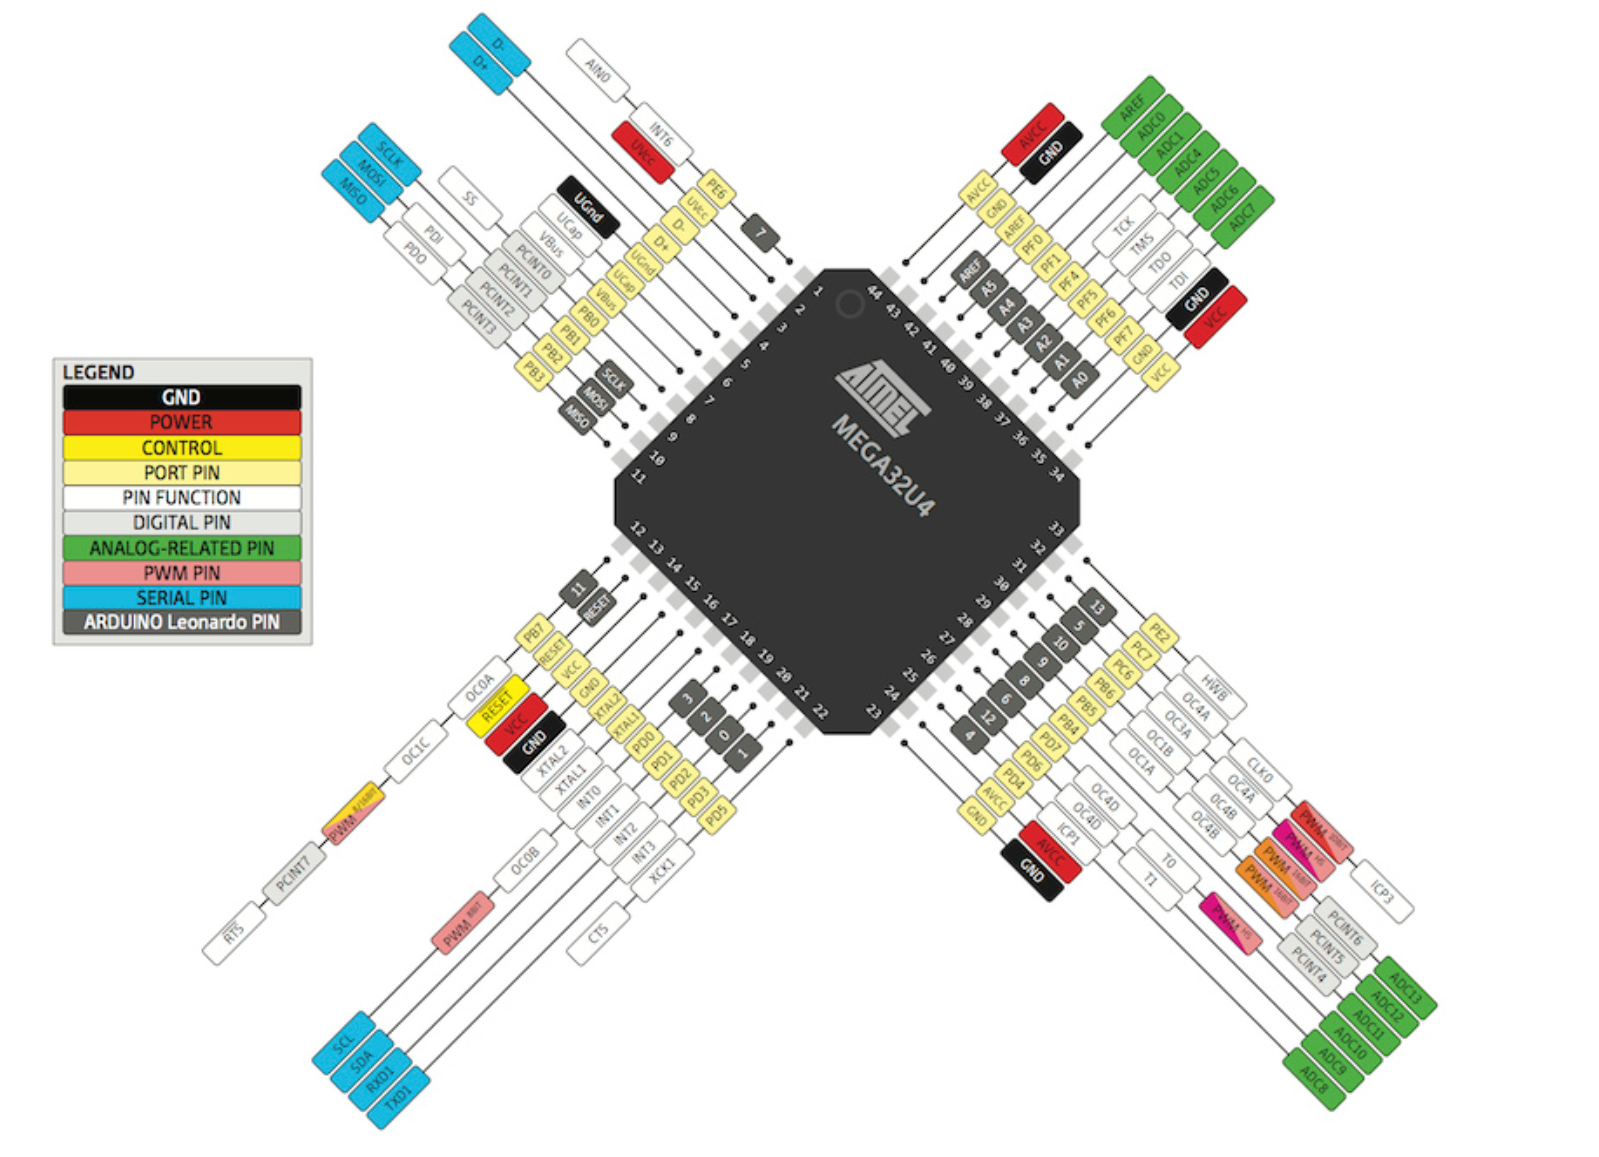
\includegraphics[width=1\textwidth]{figuras/fig-atmega32u4-pinout.png}
		\caption{\textit{ATmega32U4} pinout \cite{atmega32u4-pinout}}
		\label{fig:atmega32u4-pinout}
	\end{figure}
		

	\subsection{MCU circuit}\label{ssec:mcu-circuit}

		This MCU is the same used on the Arduino Leonardo Board \cite{arduino-leonardo}, whereas, in order to avoid implementation problems the MCU peripheral components were choosen based on the Arduino board schematic \cite{arduino-leonardo-schematic}. The circuit with all the peripheral components to the ATmega32U4 can be divided in five parts.

		\subsubsection{Core Circuit}\label{sssec:core-circuit}
			Figure \ref{fig:mcu-core-circuit} shows the core circuit for the MCU.

			\begin{figure}[htbp]
				\centering
				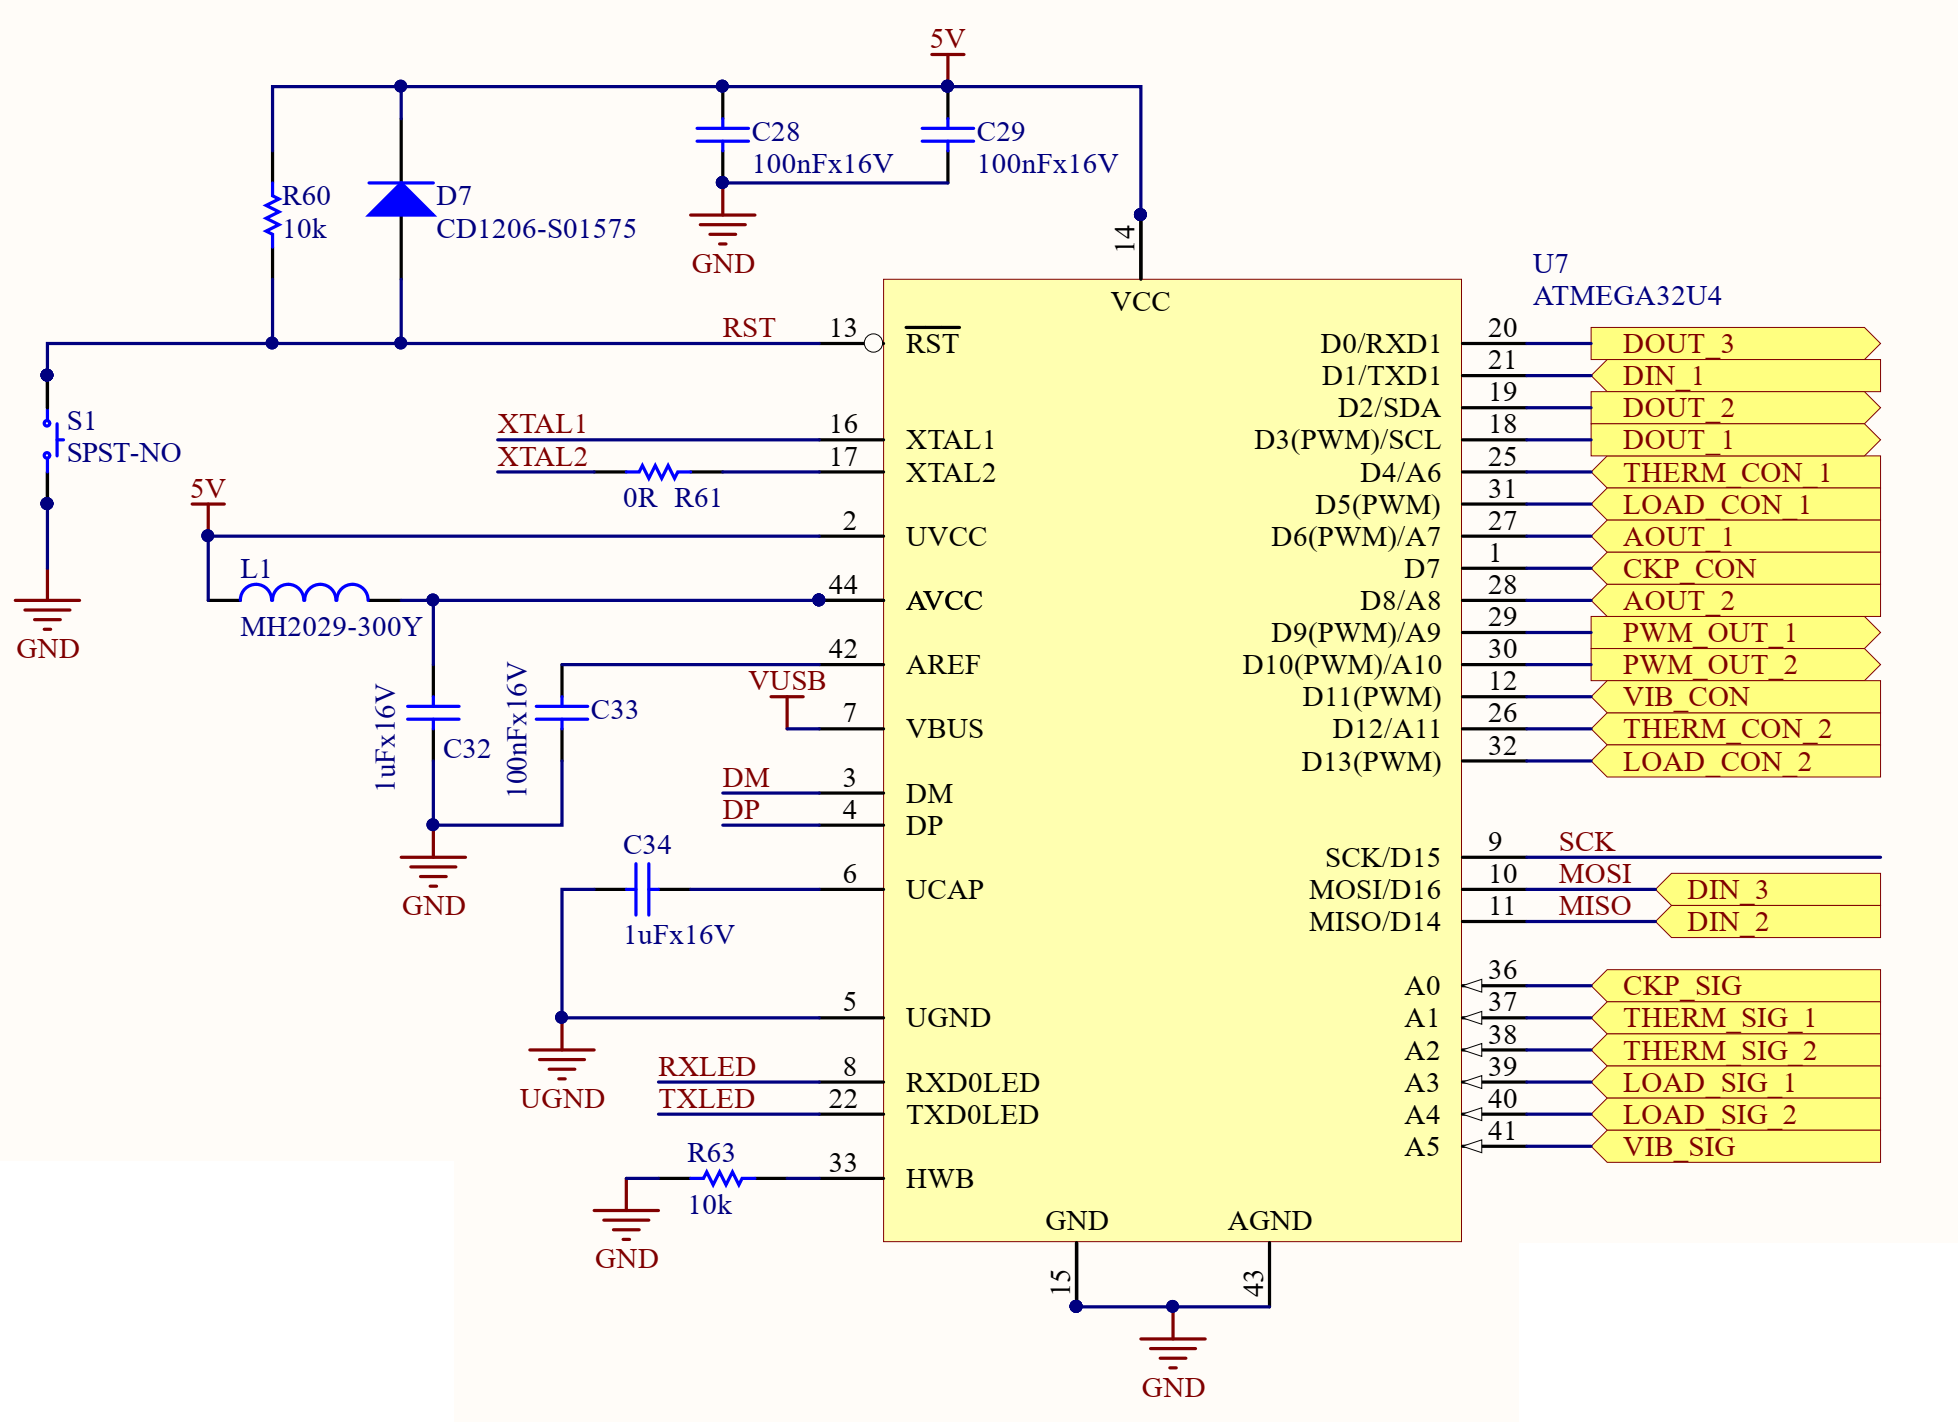
\includegraphics[width=1\textwidth]{figuras/fig-mcu-core-circuit}
				\caption{MCU Core Circuit}
				\label{fig:mcu-core-circuit}
			\end{figure}

			The components of his circuit and their respective functions are:

			\begin{itemize}
				\item\textit{U7}: The ATmega32U4 chip itself.
				\item\textit{C28 and C29}: This are bypass capacitors recommended by the datasheet.
				\item\textit{S1, D7 and R60}: RST is the reset pin of the MCU, it resets the MCU when low logic voltage is detected. S1 is a push-button used to short circuit the RST pin to ground and reset the MCU. R60 is a pull-resistor used to guarantee that RST pin will remain in high logic voltage when the push-button is not being pressed. 
				\item\textit{R61:} This jumper will be explained in Section \ref{sssec:crystal-oscillator-circuit}.\label{itm:crystal-oscillator-jumper}
				\item\textit{L1 and C32}: This components form a LPF for the AVCC pin, which is the power supply for the MCUs ADC.
				\item\textit{C33 and C34}: Both are bypassing capacitors recommended by the datasheet, C33 for the ADC internal voltage supply and C34 for the USB 2.0 controller.
				\item\textit{R63}: It is a pull-down resistor that enables hardware boot.
			\end{itemize}

			The MCU ports were defined as the following:

			\begin{itemize}
				\item\textit{DOUT$\_$1, DOUT$\_$2 and DOUT$\_$3}: Digital Output ports	
				\item\textit{DIN$\_$1, DIN$\_$2 and DIN$\_$3}: Digital input ports.
				\item\textit{CKP$\_$SIG, THERM$\_$SIG$\_$1, THERM$\_$SIG$\_$2, LOAD$\_$SIG$\_$1, LOAD$\_$SIG$\_$2 and VIB$\_$SIG}: Those are respectively the analog input ports for the signal of: speed sensor, first temperature sensor, second temperature sensor, first force sensor, second force sensor, cibration sensor.
				\item\textit{CKP$\_$CON, THERM$\_$CON$\_$1, THERM$\_$CON$\_$2, LOAD$\_$CON$\_$1, LOAD$\_$CON$\_$2 and VIB$\_$CON}: Those are digital inputs used to detect if one of the sensors from the previous item were disconnected.
				\item\textit{PWM$\_$OUT$\_$1, AOUT$\_$1, PWM$\_$OUT$\_$2 and AOUT$\_$2}: Those are respectively: first PWM output, MCU analog input to monitor the first system analog output, second PWM output, MCU analog input to monitor the second system analog output.
				\item\textit{SCK, MOSI and MISO}: Those are signal used to program the MCU through ISP(In System Programming).
				\item\textit{XTAL1 and XTAL2}: Respectively the input and output for the crystal oscilator circuit.
				\item\textit{VUSB}: This is the suppy voltage pin for the USB controller, it is being powered by a external USB host connected to the board.
				\item\textit{DM and DP}: USB data lines.
				\item\textit{RXLED and TXLED}: Pins that goes to low logic level when data is being transmitted and high logic level when not.
			\end{itemize}

		\subsubsection{Crystal Oscillator Circuit}\label{sssec:crystal-oscillator-circuit}
			According to \cite{atmega32u4-datasheet}, in order to work in full-speed mode, the MCU needs a external crystal oscillator with a frequnecy of 8 to 16MHz and bypassing capacitors from 12 to 22pF on the crystal pins. Based on \cite{arduino-leonardo-schematic} besides this capacitor a 1M$\Omega$ bias resistor has been placed between crystal pins. Also a 0R jumper (first mentioned in Item \ref{itm:crystal-oscillator-jumper} from Section \ref{ssec:mcu-circuit} was placed between one of the crystal pins and pin XTAL2 in case a low pass filter is needed (using this resistor and the internal capacitance of the MCU port). The desined circuit for the crystal oscillator is shown in Figure \ref{fig:crystal-oscillator-circuit} (except for the 0R jumper which can be seen in Figure \ref{fig:mcu-core-circuit}.

			\begin{figure}[htbp]
				\centering
				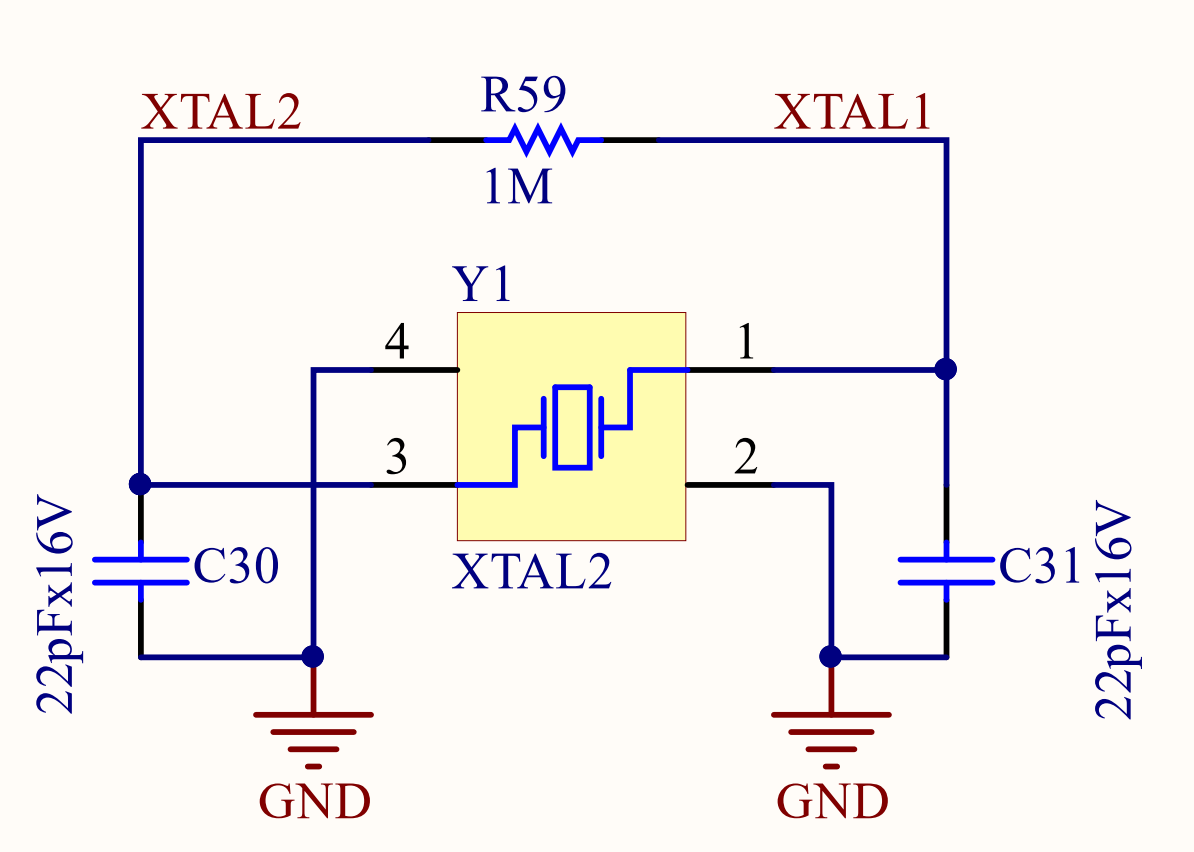
\includegraphics[width=.6\textwidth]{figuras/fig-crystal-oscillator-circuit}
				\caption{Crystal Oscillator Circuit}
				\label{fig:crystal-oscillator-circuit}
			\end{figure}
			

		\subsubsection{USB Port Protection Circuit}\label{sssec:usb-port-protection}
			The USB Port Protection circuit was entirely based on the on the circuit from Arduino Leonardo, the only component specified by the MCU datasheet are the 22$\Omega$ series resistors as shown in Figure \ref{fig:usb-port-protection-circuit}.

			\begin{figure}[htbp]
				\centering
				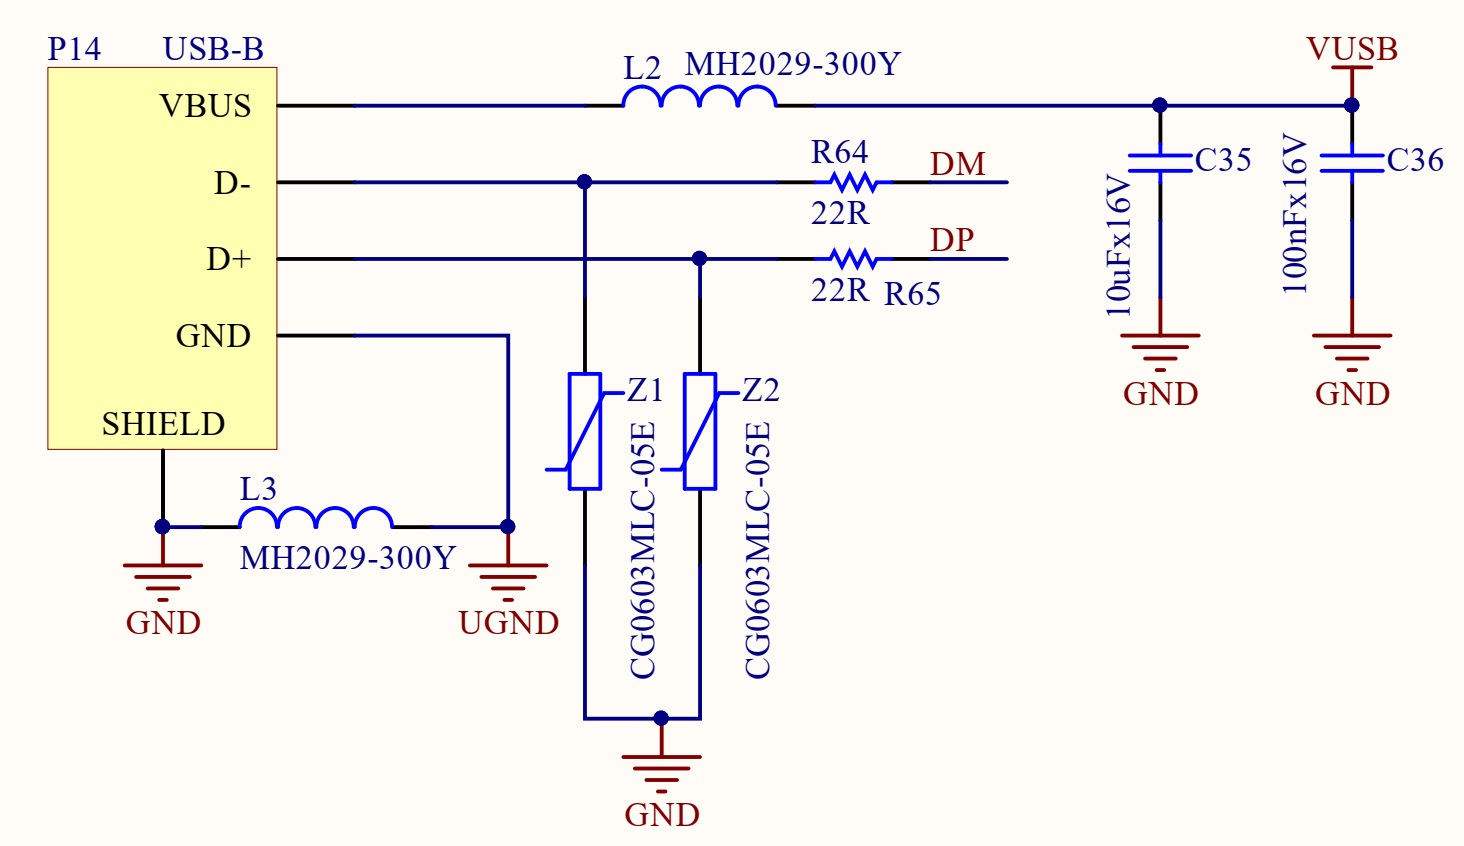
\includegraphics[width=.8\textwidth]{figuras/fig-usb-port-protection-circuit}
				\caption{USB Port Protection Circuit}
				\label{fig:usb-port-protection-circuit}
			\end{figure}

			L2 and L3 are ferrite beads used to filter high frequency noise. Z1 and Z2 are ESD supressors, alongside with the series resistors used to protect the MCU's USB data lines. Finally, C35 and C36 are bypass capacitors used to stabilize the voltage on the USB power line.